%--------------------------------------------------------------------------------------
% Dokumentum formátuma [Document format]
%--------------------------------------------------------------------------------------

\documentclass[12pt,a4paper,oneside]{report}             % Egyoldalas [Single-side]
%\documentclass[12pt,a4paper,twoside,openright]{report}  % Kétoldalas [Duplex]


%--------------------------------------------------------------------------------------
% Csomagok inicializálása [Initializing packages]
%--------------------------------------------------------------------------------------
\input{include/packages}


%--------------------------------------------------------------------------------------
% Dokumentum nyelve [Language]
%--------------------------------------------------------------------------------------

\input{include/language-setup-hu} % Beállítások magyar nyelvű dolgozathoz

% Megjegyzés: 
%         Ez a beállítás az automatikusan létrehozott címek, hivatkozások
%         nyelvét adja meg, valamint a nyelvre jellemző behúzási távolságot
%         használja a bekezdések elején.
%
% Note: 
%         This setting controls the language of generated titles and citations,
%         moreover the paragraph indentation.


%--------------------------------------------------------------------------------------
% Preambulum (LaTeX beállítások, makrók) [Preamble (LaTeX settings)]
%--------------------------------------------------------------------------------------
\input{include/preamble}


%--------------------------------------------------------------------------------------
% Munkatípus [Thesis type]
%--------------------------------------------------------------------------------------

\selectmsc   % Diplomaterv [Master's]


%--------------------------------------------------------------------------------------
% Változók beállítása [Setting variables]
%--------------------------------------------------------------------------------------

%TODO Állítsd be az alábbi változókat [Set these variables]

% Szerző [Author]
\def\authorFamilyName{Bodnár}
\def\authorGivenName{Bence Tibor}
\def\neptun{H2JC4M}

% Konzulens 1 [Consulent 1]
\def\consulentATitle{}
\def\consulentAFamilyName{Dudás}
\def\consulentAGivenName{Dávid}
\def\consulentARank{óraadó}

% Konzulens 2 [Consulent 2], ha nincs hagyd üresen
\def\consulentBTitle{}
\def\consulentBFamilyName{}
\def\consulentBGivenName{}
\def\consulentBRank{}

% Konzulens 3 [Consulent 3], ha nincs hagyd üresen 
\def\consulentCTitle{}
\def\consulentCFamilyName{}
\def\consulentCGivenName{}
\def\consulentCRank{}

% Témavezető
\def\supervisorTitle{dr.~}
\def\supervisorFamilyName{Budai}
\def\supervisorGivenName{Csaba}
\def\supervisorRank{adjunktus}

% Dolgozat címe [Thesis title]
\def\thesisTitle{Hat szabadsági fokú telemanipulátor fejlesztése sebészeti eszközök számára}

% Kulcsszavak (a PDF-be) [Keywords (to PDF)]
\def\keywords{mechatronika, szabályozástechnika, robotika, 5G, ipar 4.0}

% Tanszék [Department]
\def\department{\bmemogi}

%TODO Cseréld le a figures/tanszek_logo.pdf képet a tanszéked logójára!
%     [Replace figures/tanszek_logo.pdf with the logo of your department]

% Elzártan kezelendő dolgozat [Restricted access]
%TODO Töltsd ki a korlátozás lejártának dátumát! 
%     [Fill in the end date of the restriction]
\def\endOfRestrictedAccess{... év ... hónap ... nap}


% Változók beállítása a PDF fájlhoz [Apply variables for the PDF file]
\applyvariables


%--------------------------------------------------------------------------------------
% Dokumentum törzse [Document body]
%--------------------------------------------------------------------------------------

\begin{document}

\pagenumbering{gobble}
\selectthesislanguage

% Címoldal [Titlepage]
\include{include/titlepage-thesis}  % Szakdolgozat/Diplomaterv címlap [Thesis]

\include{include/copyrightpage}               % Nyílt kezelésű [Open access]



% Feladatkiírás [Project page]
%TODO A nyomtatott verzóban ne szerepeljen! [Remove before printing]
%--------------------------------------------------------------------------------------
% Feladatkiiras (a tanszeken atveheto, kinyomtatott valtozat)
%--------------------------------------------------------------------------------------
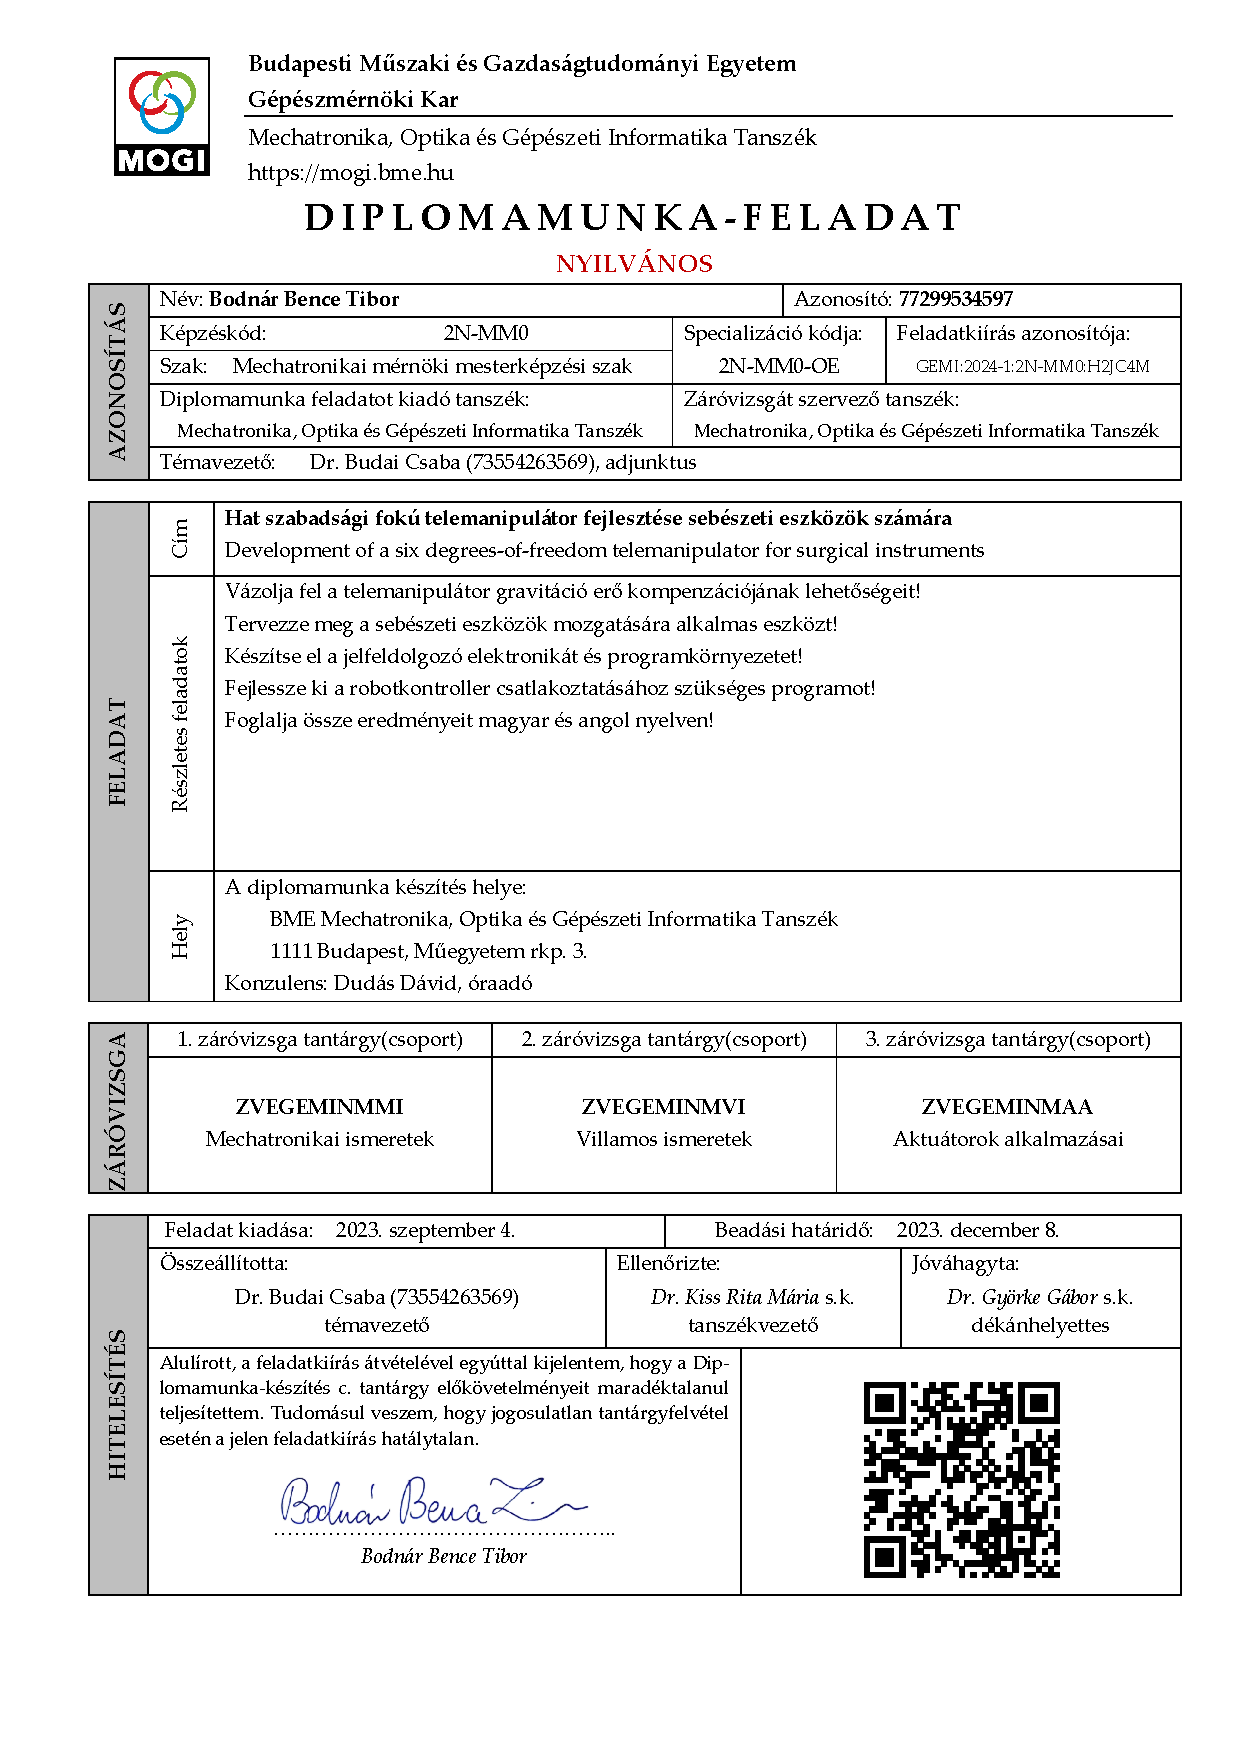
\includepdf[pages=-]{include/MOGI_DM_H2JC4M_23o.pdf}




% Nyilatkozatok [Declarations]
\selectlanguage{magyar}
\selecthungarian
\pagenumbering{roman}
\setcounter{page}{6}
\cleardoublepage % duplexnél páratlan oldalon legyen
%--------------------------------------------------------------------------------------
% Nyilatkozatok
%--------------------------------------------------------------------------------------
\begin{center}
\section*{NYILATKOZAT}
\end{center}

\vspace{0.5cm}

\begin{center}
\emph{Nyilatkozat az önálló munkáról}
\end{center}
Alulírott,  \emph{\authorFamilyName{} \authorGivenName} (\neptun), a Budapesti Műszaki és Gazdaságtudományi Egyetem hallgatója, büntetőjogi és fegyelmi felelősségem tudatában kijelentem és sajátkezű aláírásommal igazolom, hogy ezt a \MakeLowercase{\gpkmunkatipustHU} meg nem engedett segítség nélkül, saját magam készítettem, és dolgozatomban csak a megadott forrásokat használtam fel. Minden olyan részt, melyet szó szerint vagy azonos értelemben, de átfogalmazva más forrásból átvettem, egyértelműen, a hatályos előírásoknak megfelelően, a forrás megadásával megjelöltem.

\begin{flushleft}
Budapest, \today
\end{flushleft}

\begin{flushright}
 \makebox[7cm]{\rule{6cm}{.4pt}}\\
 \makebox[7cm]{\emph{hallgató}}
\end{flushright}


\vfill
\clearpage

\selectthesislanguage

\newcounter{romanPage}
\setcounter{romanPage}{\value{page}}
\stepcounter{romanPage}


\selectthesislanguage
% Tartalomjegyzék [Table of Contents]
\setcounter{tocdepth}{3}  % Tartalomjegyzék mélysége [ToC depth]
\tableofcontents\vfill


% Ábrák és táblázatok jegyzéke [List of Figures, Tables]
%TODO Kommenteld ki, ha használni szeretnéd. [Uncomment to use]
%\listoffigures\addcontentsline{toc}{chapter}{\listfigurename}   % Ábrák jegyzéke - opcionális
%\listoftables\addcontentsline{toc}{chapter}{\listtablename}     % Táblázatok jegyzéke - opcionális


% Előszó [Preface]
%----------------------------------------------------------------------------
\chapter*{\eloszo}\addcontentsline{toc}{chapter}{\eloszo}
%----------------------------------------------------------------------------

Az előszó legtöbbször személyes hangú, eligazító jellegű írás, amely a mű megírásának okairól, születésének körülményeiről szól. Az előszó nem szerves része a főszövegnek, hanem annak kiegészítése.
Ugyancsak az előszóban fejtheti ki a szerző a mű megértéséhez szükséges szempontokat, a követett módszereket, utalhat a fontosabb előzményekre és szakirodalomra.
Az előszó ne legyen terjedelmes.


Jelen dokumentum egy diplomaterv-sablon, amely formai keretet ad a BME Gépészmérnöki Karán végző hallgatók által elkészítendő szakdolgozatnak és diplomatervnek. A sablon használata opcionális. Ez a sablon \LaTeX~alapú, a \emph{TeXLive} \TeX-implementációval és a PDF-\LaTeX~fordítóval működőképes.
A sablon forrása a Mechatronika Szakosztály GitHub tárhelyén\footnotemark{} elérhető. Amennyiben hibát találtál, vagy észrevételed, javaslatod lenne, kérlek ott jelezd.

\footnotetext{\url{https://github.com/MechatronikaSzakosztaly/bme-gpk-thesis-latex}}

\begin{center}
    $\thicksim \; \thicksim \; \thicksim$
\end{center}


\subsubsection*{Köszönetnyilvánítás}
\emph{Szeretnék köszönetet mondani témavezetőmnek, Dr. Budai Csabának és a konzulensemnek Dudás Dávidnak a több féléves munkájáért. Szeretném megköszönni Dr. Bodnár Tibor, Bodnárné Dr. Gyarmathy Dórának és Dr. Gyarmathy Miklósnénak a támogatást és a lektorálást. Szeretnék köszönetet mondani Dr. Kiss Rita tanészékvezető asszonynak és tanészékének a támogatásért. Szeretném megköszönni az Orvostechnika Szakosztály tagjainak a projektben vállalt kisebb feladatokban nyújtott segítséget, illetve a lehetőséget, hogy ezzel a projekttel hozzájárulhattam a Szakosztály életéhez.} 


\vspace{0.5cm}

\begin{flushleft}
{Budapest, \today}
\end{flushleft}

\begin{flushright}
\emph{\authorName}
\end{flushright}

\vfill



% Jelölések jegyzéke [Table of Symbols]
\newcommand{\tss}{\textsuperscript}     % tss = felső index
%----------------------------------------------------------------------------
\chapter*{\jelolesek}\addcontentsline{toc}{chapter}{\jelolesek}
%----------------------------------------------------------------------------

A táblázatban a többször előforduló jelölések magyar és angol nyelvű elnevezése, 
valamint a fizikai mennyiségek esetén annak mértékegysége található. Az egyes 
mennyiségek jelölése – ahol lehetséges – megegyezik hazai és a nemzetközi 
szakirodalomban elfogadott jelölésekkel. A ritkán alkalmazott jelölések 
magyarázata első előfordulási helyüknél található.

%~~~~~~~~~~~~~~~~~~~~~~~~~~~~~~~~~~~~~~~~~~~~~~~~~~~~~~~~~~~~~~~~~~~~~~~~~~~~~~~~~~~~~
% A táblázatokat ABC rendben kell feltölteni, először mindig a kisbetűvel
% kezdve. Ha egyazon betűjelnek több értelmezése is van, akkor mindegyiket kü-
% lön sorban kell feltüntetni. Konstansok esetén az értéket is a táblázatba
% kell írni.
% Dimenzió nélküli mennyiségek mértékegysége 1 és nem: – !
% A jelölésjegyzékben csak SI vagy SI-n kívüli engedélyezett mértékegységeket
% szabad feltüntetni. Egy dokumentumon belül az SI és pl. az angolszász
% mértékrendszer nem keverhető!
%~~~~~~~~~~~~~~~~~~~~~~~~~~~~~~~~~~~~~~~~~~~~~~~~~~~~~~~~~~~~~~~~~~~~~~~~~~~~~~~~~~~~~

%~~~~~~~~~~~~~~~~~~~~~~~~~~~~~~~~~~~~~~~~~~~~~~~~~~~~~~~~~~~~~~~~~~~~~~~~~~~~~~~~~~~~~
% A Jelölés oszlop alapvetően kurzív betűváltozattal szedendő, a Mértékegység
% oszlopot álló betűkkel kell szedni. Felső indexhez használható a \tss{}
% parancs.
%~~~~~~~~~~~~~~~~~~~~~~~~~~~~~~~~~~~~~~~~~~~~~~~~~~~~~~~~~~~~~~~~~~~~~~~~~~~~~~~~~~~~~

\def\arraystretch{1.5}%  vertical cell padding

\subsubsection*{Latin betűk}
\begin{center}
    \begin{tabular}{lp{10cm}l}
        \hline
        Jelölés & Megnevezés, megjegyzés, érték & Mértékegység   \\ 
        \hline
        $g $       & gravitációs gyorsulás         & $m / s^{2}$\\
        $t $       & idő                           & ms \\
        $m $       & tömeg                         & g  \\
        $d $       & átmérő                        & mm \\
        $h $       & hosszúság                     & mm \\
        $v $       & falvastagság                  & mm \\
        \hline
    \end{tabular}    
\end{center}



\subsubsection*{Görög betűk}
\begin{center}
    \begin{tabular}{lp{10cm}l}
        \hline
        Jelölés & Megnevezés, megjegyzés, érték & Mértékegység \\ 
        \hline
        $\alpha$   & szög                   & $\circ$        \\
        $\theta$   & szög                   & $\circ$        \\
        $\beta$    & szög                   & $\circ$        \\
        $\gamma$   & szög                   & $\circ$        \\
        \hline
    \end{tabular}
\end{center}



\subsubsection*{Indexek, kitevők}
\begin{center}
    \begin{tabular}{lp{12.8cm}}
        \hline
        Jelölés & Megnevezés, értelmezés\\ 
        \hline
        $i$     & általános futóindex (egész szám)   \\
        max     & maximális (nominális) érték        \\
        min     & minimális (nominális) érték        \\        
        \hline
    \end{tabular}    
\end{center}


\def\arraystretch{1}%  vertical cell padding



% Főszöveg [The main part of the thesis]
\cleardoublepage
\pagenumbering{arabic}
%TODO Importáld a saját fejezeteidet [Import your own content]
%----------------------------------------------------------------------------
\chapter{\bevezetes}
%----------------------------------------------------------------------------

A diploma dolgozatomban részletesen bemutatom a telemanipulátor megtervezését. A feladat, amit ehhez el kellett végeznem egy sokrétű prototípusokon alapuló rekurzív tervezési folyamat. Nehezen lehet a mérnöki életben próba, prototípus tesztelés nélkül elméleti számításokon alapuló rendszerekről következtetéseket levonni. A dolgozat tárgyát képező telemanipulátor prototípusának tekinthető a szintén általam készített szakdolgozatomban bemutatott telemanipulátor. Annak az eszköznek az elkészülését követően is számtalan ötlet és kérdés merült fel bennem, hogy hogy tudtam volna jobban elkészíteni. A diplomamunkám feladatainak megfogalmazásának idejére már egyértelművé vált számomra, hogy ugyan ezzel a témával szeretnék foglalkozni. Célom lett ezzel egy még jobb rendszert elkészíteni kiegészítve új funkciókkal.

A nehézségi erőből fakadó tehetetlenség kompenzációjának kérdése már foglalkoztatott a szakdolgozatom alatt is, de ott sajnos időhiány miatt nem sikerült elmélyednem benne, ezért kézen fekvő volt a diplomamunkám során ezzel kezdeni. Fontosnak tartottam azt, hogy a sebészeti eszközök mozgatása legyen itt is a cél, ami felé orientálódnom kell, mivel ez a terület nagy fokú precizitást és körültekintést igényel és számtalan mérnöki kihívást tartogat. Ezt követően elkezdtem megtervezni az eszközt. A tervezés során minden nagyobb módosítás vezetett el mindig a következő lépcsőfokhoz, amiknél szinte kivétel nélkül prototípus tesztelést csináltam. Igyekszem a dolgozatomban lényegre törően megfogalmazni azokat az elvárásokat, amiket minden egyes helytelen irányú tervezésnél vagy hibás következetesénél megfogalmaztam.

A következő fejezetekben a diplomamunkám során elvégzett munkámat mutatom be. Igyekszem logikailag az építési sorrendre való tekintettel felbontani a teljes feladatot és lépésről-lépésre részletesen bemutatni minden kapcsolódó technikai részletet és döntést, mit miért és mire használtam. Az előbb említettek alapján röviden elemzem a szakdolgozatomban bemutatott telemanipulátort és azokat az elvárásokat amik alapján újra terveztem az egész eszközt. A valós tervezés megkezdése előtt a gravitációs hatásából származó terhelés kompenzációjának lehetőségeit mutatom be és extra elvárásként fogalmazom meg, hogy a tervezésnek figyelembe kell vennie ennek megvalósíthatóságát is. Ezt követően az elvárások figyelembe vételével a geometriai kialakítást, az jelfeldolgozó rendszert és a hozzátartozó mikrovezérlő programot megvalósítását részletezném. Végül pedig a kész telemanipulátorral gyűjtött adatok feldolgozását és felhasználásának módját mutatnám be, amivel szimulációs majd valós robotkart is célom vezérelni.      % Bevezetés
%----------------------------------------------------------------------------
\chapter{Munkám során használt eszközök}
\label{sec:LatexTools}
%----------------------------------------------------------------------------
\section{Direkt kinematika}
%----------------------------------------------------------------------------
A direkt kinematika és a Khali-féle Denavit-Hartenberg (DH) módszer a robotika területén alkalmazott módszerek, amelyek lehetővé teszik a robotkarok és manipulátorok mozgásterének és pozíciójának meghatározását. Az alábbiakban bemutatom ezeket a módszereket és azok fő jellemzőit.

A direkt kinematika a robotkarok mozgásterének és végpontjainak pozíciójának meghatározását vizsgálja. Célja, hogy a robotkar ízületeinek állapotából vagy koordináta rendszeréből kiindulva meghatározza a végpont vagy a szerszám pozícióját a világkoordináta rendszerben. Ez a módszer matematikai modelleket és transzformációkat használ a kar szegmenseinek és ízületeinek geometriájának leírására és kapcsolatának meghatározására.

A Khali-féle DH módszer a direkt kinematika egyik legelterjedtebb módszere, amelyet a Denavit-Hartenberg (DH) paraméterek felhasználásával végeznek. Ez a módszer egy koordináta rendszer hierarchikus láncolását használja a robotkar szegmensei közötti kapcsolat leírására. A DH módszerben a kar szegmenseinek geometriáját és relatív helyzetét négy paraméter segítségével írják le: az alfa, a, d és theta paraméterek.

Az alfa paraméter az aktuális ízület tengelyének elfordulását jelenti a szomszédos szegmens tengelyéhez képest. Az a paraméter a szegmens hosszát vagy az ízület távolságát jelenti az előző szegmenstől. A d paraméter a szegmens központjának távolságát jelenti az előző szegmenstől a közös tengely mentén. A theta paraméter pedig az aktuális ízület elfordulását jelenti.

A DH módszerben minden szegmenst leíró paramétert és transzformációs mátrixot alkalmaznak, amelyek segítségével a végpont pozícióját határozzák meg. A módszer iteratív módon alkalmazható, a végponttól visszafelé haladva az egyes ízületek állapotának és pozíciójának meghatározására.

A direkt kinematika és a DH módszer széles körben alkalmazott eszközök a robotika területén. Segítségükkel lehetőség nyílik a robotkarok mozgásának tervezésére, szimulációjára és vezérlésére. Ezen módszerek alkalmazásával pontosan meghatározható a robotkar végpontjának helyzete és orientációja a világkoordináta rendszerben, ami fontos információ lehet a munkafolyamatok tervezésében és végrehajtásában.

Összességében a direkt kinematika és a Khali-féle DH módszer lehetővé teszik a robotkarok mozgásterének és pozíciójának meghatározását. Ezek a módszerek alapvetőek a robotika területén, és fontos szerepet játszanak a robotkarok tervezésében, szimulációjában és vezérlésében. A direkt kinematika és a DH módszer segítségével precízen modellezhetők és kontrollálhatók a robotkarok mozgásai, amelyek számos ipari és egyéb alkalmazásban hasznosak lehetnek.

\section{Inverz kinematika}
%----------------------------------------------------------------------------
Az inverz kinematika a robotika területén használt módszer, amely lehetővé teszi a robotkarok számára, hogy meghatározzák az ízületeik állapotát és pozícióját a kívánt végpont vagy TCP (tool center point) eléréséhez. Ez a módszer a direkt kinematika ellentéte, mivel itt nem a végpont pozícióját kell meghatározni az ízületek ismert állapota alapján, hanem éppen fordítva: az ízületek állapotát kell meghatározni a kívánt végpont pozíciója alapján.

Az inverz kinematika alkalmazása során a robotkar rendszerének geometriáját és ízületeinek korlátait figyelembe véve meg kell határozni az ízületek szögét vagy állapotát, amelyekkel a TCP a kívánt pozícióba kerül. Ez egy matematikai probléma, amelyet általában numerikus vagy analitikus megoldó algoritmusok segítségével oldanak meg.

Az inverz kinematika számos alkalmazási területtel rendelkezik a robotikában. Például a gyártósorokon, ahol a robotkaroknak pontosan kell pozícionálniuk a szerszámokat vagy alkatrészeket, az inverz kinematika segítségével a kívánt végpont pozíció alapján meg lehet határozni az ízületek állapotát. Ez lehetővé teszi a robotkarok pontos és ismételhető mozgását a gyártási feladatok hatékony végrehajtása érdekében.

A Khali-féle DH módszer a robotkarok leírására és az inverz kinematika alkalmazására is használt módszer. Ennek során a robotkar ízületeinek és szegmenseinek geometriáját és kapcsolatát a Denavit-Hartenberg (DH) paraméterek segítségével írják le. Ezek a paraméterek az alfa, a, d és theta értékekből állnak, amelyek meghatározzák az ízületek elfordulását és a szegmensek geometriáját.

A DH paraméterekkel leírt robotkar geometriáját felhasználva a Khali-féle DH módszerrel meghatározható az inverz kinematika. Az algoritmus segítségével a kívánt végpont vagy TCP pozíciója alapján a szükséges ízületi szög vagy állapot meghatározható. Az így kapott eredményeket a robotvezérlő egység továbbítja a robotkar motorjainak, hogy a megfelelő pozícióba mozgassa a TCP-t.

Az inverz kinematika és a Khali-féle DH módszer együttműködve lehetővé teszik a robotkarok számára, hogy a kívánt végpont vagy TCP pozíciókba helyezkedjenek el. Ez kulcsfontosságú a precíz munkavégzéshez és a különböző feladatok hatékony végrehajtásához a robotika számos alkalmazási területén, például az ipari automatizációban, a gyártásban, a logisztikában és a sebészeti beavatkozásokban. Az inverz kinematika és a Khali-féle DH módszer jelentős fejlődést hozott a robotkarok irányításában és pozícionálásában, és további lehetőségeket teremt a robotika területén.

\section{ROS}
%----------------------------------------------------------------------------
A Robot Operating System, röviden ROS, egy nyílt forráskódú, rugalmas és elosztott szoftverrendszer, amelyet a robotok fejlesztéséhez és irányításához használnak. Az alábbiakban összefoglalom a ROS rendszert, kitérve a node-okra, a topic-okra és a robotrendszerekben történő alkalmazásukra.

A ROS egy gráfalapú rendszer, amelyben a különböző komponenseket, úgynevezett node-okat, összekapcsolják egymással, hogy információt és parancsokat cseréljenek. A node-ok önálló folyamatok, amelyek futnak és kommunikálnak egymással. Minden node specifikus feladatokat lát el, például szenzoradatok gyűjtése, adatfeldolgozás, irányítás vagy más műveletek végzése.

A node-ok közötti kommunikáció a topic-okon keresztül történik. A topic egy adatcsatorna, amely lehetővé teszi a node-ok közötti aszinkron adatátvitelt. Egy node publikálhat adatokat egy topic-ra, és más node-ok feliratkozhatnak erre a topic-ra, hogy megkapják az adatokat. Ez a központi kommunikációs mechanizmus a ROS rendszerben. Például egy szenzor node adatokat publikálhat egy "lidar" nevű topic-ra, és egy navigációs node feliratkozhat erre a topic-ra, hogy megkapja a szenzoradatokat és használhassa őket a robot navigációjához.

A ROS rendszer különösen népszerű a robotrendszerek fejlesztésében és irányításában. A robotok általában több szenzorral rendelkeznek, amelyek adatokat gyűjtenek a környezetről, például távolság, helyzet, kép vagy hanginformációk. Ezeket a szenzoradatokat a ROS node-ok gyűjtik és feldolgozzák. Emellett a robotoknak vezérlési parancsokat kell fogadniuk és végrehajtaniuk. A ROS lehetővé teszi a vezérlő node-ok létrehozását, amelyek az irányítást végzik, például a robot mozgását vagy más műveleteit vezérlik.

A ROS rendszerben a node-ok és topic-ok rugalmasan konfigurálhatók és összekapcsolhatók, ami lehetővé teszi a fejlesztők számára a moduláris és újrafelhasználható szoftverkomponensek létrehozását a robotalkalmazásokhoz. Ez a moduláris szerkezet elősegíti a fejlesztés hatékonyságát, és lehetővé teszi a különböző csapatok számára, hogy párhuzamosan dolgozhassanak az egyes részegységeken.

Összességében a ROS egy erőteljes és rugalmas szoftverrendszer, amely lehetővé teszi a fejlesztők számára a robotrendszerek fejlesztését és irányítását. A node-ok és topic-ok használata lehetővé teszi az adatok gyűjtését, feldolgozását és megosztását a rendszer komponensei között, ezáltal segítve a robotok működését és irányítását különböző feladatok végrehajtása során.

\section{STM32 nucleo}
%----------------------------------------------------------------------------
A Cortex-M4 egy ARM architektúrájú processzormag, amelyet beágyazott rendszerekhez terveztek. A Cortex-M4 processzormagok nagy teljesítményt és alacsony energiafogyasztást kínálnak, és széles körben elterjedtek az ipari, gyártási és beágyazott alkalmazások területén.

Az STM32 fejlesztőeszközök a Cortex-M4 processzormaggal rendelkező STM32 mikrovezérlők családjára épülnek. Az STM32 mikrovezérlők az STMicroelectronics által gyártott nagyon népszerű és széles körben használt beágyazott rendszerekre szánt eszközök. Az STM32 fejlesztőeszközök kiváló minőségű hardvereket és szoftvereszközöket kínálnak a fejlesztőknek a STM32 mikrovezérlők programozásához és teszteléséhez.

A NUCLEO-F411RE board egy konkrét példa az STM32 fejlesztőeszközök közül. Ez a fejlesztői platform az STM32F411RE mikrovezérlőre épül, amely egy Cortex-M4 processzormaggal rendelkező mikrovezérlő. A NUCLEO-F411RE board kiváló választás azok számára, akik be szeretnének vezetődni az STM32 világába és megismerkedni az ARM Cortex-M4 alapú fejlesztéssel.

A NUCLEO-F411RE board számos funkcióval és interfésszel rendelkezik, ideértve digitális és analóg bemeneteket, PWM kimeneteket, UART, I2C, SPI és USB interfészeket, valamint egy ST-Link programozó/debugger egységet. Ez a board könnyen használható és támogatja a fejlesztőket az alkalmazásaik prototípusolásában, fejlesztésében és tesztelésében.

Az STM32 fejlesztőeszközökön általában kényelmesen használható fejlesztői környezet, például az STM32CubeIDE vagy az STM32CubeMX áll rendelkezésre. Ezek az eszközök számos fejlesztői funkciót és eszközt biztosítanak, például kódszerkesztőt, kódgenerátort, szimulációs lehetőségeket és debugger eszközöket, hogy segítsék a fejlesztőket a hatékony és könnyű fejlesztésben.

Összefoglalva, a Cortex-M4 alapú rendszerek, mint az STM32 mikrovezérlők és az ehhez kapcsolódó fejlesztőeszközök, kiváló választásnak számítanak beágyazott rendszerek tervezéséhez és fejlesztéséhez. Az STM32 fejlesztőeszközök, például a NUCLEO-F411RE board, rugalmas és hatékony platformot kínálnak a Cortex-M4 alapú alkalmazások prototípusolásához és teszteléséhez, valamint a fejlesztői folyamat megkönnyítéséhez.

\subsection{UART port}
Az "UART" rövidítés a "Universal Asynchronous Receiver/Transmitter" kifejezést takarja. Az UART egy soros kommunikációs protokoll, amely a digitális adatok átvitelét teszi lehetővé két eszköz között. Ez a protokoll olyan eszközök közötti soros kommunikációt biztosít, amelyek között nincs központi órajel (asynchronous), tehát az adatküldés és -fogadás időzítése a két eszköz között előre nem megállapodott.

Az UART általában két vezetéken keresztül történik: TX (Transmitter) és RX (Receiver). Az adatok a TX vezetéken keresztül mennek egyik eszköztől a másikig, és a RX vezetéken keresztül az ellenkező irányban. A kommunikációt start és stop bitek, valamint adatbitek alkotják.

A UART port vagy interfész tehát a hardver vagy a vezérlő, amely lehetővé teszi az UART protokollt támogató eszközök közötti kommunikációt. Az UART portok széles körben alkalmazottak például számítógépek, mikrovezérlők, beágyazott rendszerek és egyéb eszközök kapcsolódási pontjaiként. Az UART segítségével a különböző eszközök adatokat küldhetnek és fogadhatnak egymástól, amely lehetővé teszi a sokféle elektronikai eszköz közötti egyszerű és megbízható kommunikációt.

\section{GMR szenzor}
%----------------------------------------------------------------------------
A GMR (giant magnetoresistance) szenzorok olyan érzékelők, amelyeket tengelyszög elfordulásának mérésére használnak. Ezek a szenzorok a GMR technológiára támaszkodnak, amely kihasználja a mágneses mező érzékelését és lehetővé teszi a precíz és megbízható tengelyszög mérését. Ebben a kontextusban bemutatjuk a TLE5012 szenzort, amely egy népszerű és megbízható GMR szenzor a tengelyszög elfordulás mérésére.

A TLE5012 egy 2D-GMR szenzor, amely két tengelyre (X és Y) érzékeny. Ez a szenzor nagyon kicsi, integrált kivitelű és digitális interfésszel rendelkezik, amely lehetővé teszi a könnyű integrációt a különböző alkalmazásokban. A TLE5012 szenzor nagy felbontással és nagy pontossággal rendelkezik, és képes a tengelyszög elfordulásának pontos érzékelésére a mágneses mező változásán keresztül.

A TLE5012 szenzor működése az óriásmágneses ellenállás jelenségen alapul. A szenzor egy mágneses mező hatására változtatja meg az elektromos ellenállását, és ezáltal méri a tengelyszög elfordulását. A szenzor beépített ADC (Analog-to-Digital Converter) segítségével digitalizálja az érzékelt jelet, és digitális adatként továbbítja a rendszer számára. A TLE5012 szenzor nagyon gyors működést tesz lehetővé, ami ideális a valós idejű alkalmazásokhoz.

A TLE5012 szenzor nagyon sokoldalú, és számos alkalmazási területen használható. Az autóiparban gyakran alkalmazzák a kormányzás elfordulásának érzékelésére és a kormányzás rendszerének vezérlésére. Ez lehetővé teszi a jármű pontos irányítását és a vezetésbiztonság javítását. Emellett a TLE5012 szenzort gyakran alkalmazzák robotika, ipari automatizálás és egyéb beágyazott rendszerekben is, ahol a tengelyszög elfordulásának pontos mérése szükséges.

A TLE5012 szenzor könnyen integrálható a rendszerbe, és számos előnyös tulajdonsággal rendelkezik. Például a szenzor hibrid működésű lehet, ami lehetővé teszi a redundancia beépítését a megbízhatóság növelése érdekében. Emellett a TLE5012 szenzor alacsony energiafogyasztással rendelkezik, ami fontos tényező a hordozható vagy akkumulátoros eszközök esetében.

A TLE5012 szenzor rendelkezik továbbá kiterjedt konfigurációs és kalibrációs lehetőségekkel, amelyek lehetővé teszik a szenzor beállítását a konkrét alkalmazás igényei szerint. A szenzorhoz általában fejlesztői környezet és dokumentáció is tartozik, amelyek segítenek a rendszerbe történő integrációban és a megfelelő működés beállításában.

Összességében a GMR szenzorok, például a TLE5012, nagyszerű lehetőséget nyújtanak a tengelyszög elfordulásának érzékelésére. A GMR technológia kiemelkedő érzékenységet, precizitást és gyors működést kínál, amely lehetővé teszi a pontos tengelyszög mérését a különböző alkalmazásokban. A TLE5012 szenzor konkrétan számos előnyös tulajdonsággal rendelkezik, és széles körben alkalmazható az autóipartól a robotikáig és az ipari automatizálásig.
%----------------------------------------------------------------------------
\chapter{Elérhető telemanipulátorok}
\label{sec:LatexTools}
%----------------------------------------------------------------------------

A telemanipulátor egy olyan robotikai rendszer, amely lehetővé teszi egy távoli operátor számára, hogy távolról irányítsa és manipulálja a robotkarot vagy manipulátort. Ez a rendszer általában két fő részből áll: a távoli operátor konzoljából és a fizikai manipulátorból, amelyet általában egy robotkar vagy robotikai kar alkot.

A telemanipulátor rendszer célja, hogy a távoli operátor lehetőséget kapjon a távoli helyen történő munkavégzésre, amely lehet veszélyes környezet, távoli terület vagy olyan hely, ahová az ember nem férhet hozzá. A távoli operátor a konzol segítségével ad utasításokat a manipulátornak, amelyeket a robotkar vagy a manipulátor végrehajt a távoli helyen. Ennek eredményeként a távoli operátor képes manipulálni, mozgatni vagy érinteni tárgyakat a távoli helyen.

A telemanipulátorok széles körben alkalmazhatók különböző iparágakban és területeken. Például az űrkutatásban és az űrszemétszedésben használják a távoli helyen történő műveletek elvégzésére. Az orvostudományban telemanipulátorok segítségével végezhetnek távoli műtéteket és beavatkozásokat. Az ipari gyártásban használják a távoli manipulációt és a precíz munkafolyamatokat.

A telemanipulátor rendszerek különböző szenzorokat és eszközöket használnak, például képfeldolgozást, erőérzékelést és távérzékelést, hogy pontosabb és intuitívabb vezérlést biztosítsanak a távoli operátor számára. Az előrehaladó technológiák, például a virtuális valóság és a távérzékelés, további lehetőségeket kínálnak a telemanipuláció területén.

A telemanipulátor rendszerek lehetővé teszik az ember és a robot együttműködését, és hozzájárulnak a távoli helyeken történő feladatok hatékony és biztonságos elvégzéséhez. Ezáltal a telemanipuláció előnyös lehet olyan helyzetekben, ahol emberi jelenlét nem kívánatos vagy nem lehetséges, de mégis szükség van az emberi kézügyességre és irányításra.
\section{Telemanipulátorok az iparban}
%----------------------------------------------------------------------------
\section{Telemanipulátor az orvosi robotok vezérlésére}
%----------------------------------------------------------------------------
\section{Hat szabadság fokú telemanipulátor}
%----------------------------------------------------------------------------
Szakdolgozatomban bemutatott telemanipulátor egy egyszerű egytagú karokból és csuklókból összeállított eszköz. Az eszköz elkészítésének koncepciója, hogy a hatodik csuklóra helyezhető legyen egy geometria, amelynek a TCP-jának térben való elmozdulását rögzítsem a csuklószögek mérésével. Az alábbi képen is látható (\ref{fig:Szakdoga_csipeszes}) az elkészített eszköz.

\begin{figure}[!ht]
\centering
\includegraphics[width=150mm, keepaspectratio]{figures/Szakdoga/0_v_4_csipeszes}
\caption{Szakdolgozatomban elkészített telemanipuláto}
\label{fig:Szakdoga_csipeszes}
\end{figure}

Nagyon fontosnak tartottam, hogy a megtervezett eszközt el is készítsem valamilyen formában, mivel így sokkal alaposabban megtudtam vizsgálni az eszközt. A telemanipulátor 3D nyomtatással lett elkészítve. A FDM\footnote{Fused Deposition Modeling - A nyomtatási technológia a hőre lágyuló polimerekkel képes 3D-s objektumokat nyomtatni. Az FDM nyomtatók azzal az alapelvvel működnek, hogy szobahőmérsékleten szilárd hőre lágyuló polimert 180$^{\circ}$- 300$^{\circ}$C-ra melegítve ömledéket állapotba kerülnek és a kívánt helyre lehet juttatni lineáris vezetékrendszer segítségével.} technológiával készült, viszont néhány alkatrész, mint például a szenzortartó elkészítéséhez SLA\footnote{StereoLithography Apparatus - modellteret UV aktív gyantával tölti fel. A nyomtatási térben egy síklapra építi fel a tárgyat úgyhogy, az belemerül egy gyantával teli kádba, ahol a megfelelő rétegvastagságú folyékony gyanta réteget UV lézerrel térhálósítja és köti adhézióval az előző réteghez} módon működő nyomtatót használtam. 

 % 2. fejezet
\chapter{Telemanipulátor geometriája}
\label{sec:geometria}

A szakdolgozatomban elkészített telemanipulátor koncepcionális újragondolását és a kompenzációs elvárásokat az előző fejezetben bemutattam. Az elvárási szempontok figyelembevételével megterveztem a telemanipulátor geometriai vázát.

A diploma dolgozatomban bemutatásra kerülő telemanipulátor geometriájának megtervezése több féléves munka után nyerte el végső formáját. A tervezési lépéseket a kompenzáció miatt szükséges elvi felépítéstől indulva mutatom be. Végül a kinematikai felépítését és a TCP pont számításához szükséges elemzéssel zárnám a fejezetet.

%----------------------------------------------------------------------------
\section{Geometria kialakítása}
%----------------------------------------------------------------------------

A kompenzációnál megemlített paralelogramma elrendezés használata rendkívül hasznos megoldásnak bizonyult és az egyik legnagyobb fejlesztésnek tartam a szakdolgozatban dokumentált munkámhoz képest. A paralelogramma elrendezés
miatt a kábel csatornák száma az ötödik csuklóig meg kétszereződött, mivel karonként kétszer annyi elem áll rendelkezésre. Ezen túl a rendszer stabilitását is növelte az által, hogy jobban ellenáll csavaró vagy nyíró jellegű igénybe vételnek, amik a csuklókat terhelhetik. Előnyként mutatkozott ez az elrendezés akkor is amikor a számításokat végeztem, mivel a paralelogramma elrendezés azt eredményezi, hogy a minden oldala a kinematikának párhuzamos marad a vele szemköztivel. Az ötödik csuklóig így csak szinusz koszinusz számításokat és egy darab transzformációt kellett elvégeznem. Az általam elképzelt telemanipulátor kinematikai elrendezése a következő lett. A rendszer egészében $6[db]$ csuklóban mérendő szögváltozó elmozdulása alapján tudja meghatározni a TCP pontot. A elvárások alapján két darab paralelogramma kinematikai összeállítást használok és ezt követően három csuklót az end-effektorral történő mind a hat szabadsági fokon történő mozgatáshoz.

\begin{figure}[!ht]
\centering
\includegraphics[width=90mm, keepaspectratio]{figures/Diagrammok/Diploma_kinematika}
\caption{Diploma munka kinematika}
\label{fig:Diploma_kinematika}
\end{figure}

A \ref{fig:Telemnanipulátor_kinematika}.ábrán láthatóan az elkészült telemanipulátor oldalról. A képen jól látható, hogy az meghatározott kinematikai lánc teljes egészében megvalósításra került. A megvalósításnál kifejezetten nagy kihívást jelentett az, hogy a karok vastagságát milyen méretűre válasszam meg. Kinematikai váz felrajzolásánál a geometriai elemek térbeli korlátjával érthető módon nem kellett foglalkozzak viszont megvalósításánál ez korlátozó tényező már nehézséget okozott.

\begin{figure}[!ht]
\centering
\includegraphics[width=130mm, keepaspectratio]{figures/Diploma_CAD/creo2.png}
\caption{Telemnanipulátor kinematikai elrendezésének bemutatása}
\label{fig:Telemnanipulátor_kinematika}
\end{figure}

A diploma dolgozatomban már korábban is említettem, de a továbbfejleszthetőséget nagyon fontosnak tartom. A karokat úgy terveztem meg, hogy a későbbiekben ne kelljen mindenáron az egészet kicserélni, ha új koncepciós megvalósítást készítek. A következő \ref{fig:kar}.ábrán és a \ref{fig:Csuklo_egyedul}.ábrán a második és harmadik csukló közötti kar látható, illetve a kar két végén lecsavarozható idom. Az idom illeszkedik a csapágyba illetve a kar keresztmetszetén található kábel csatornát fordítja be a tengely irányába.

\begin{figure}[!ht]
\centering
\includegraphics[width=150mm, keepaspectratio]{figures/Diploma_CAD/creo3.png}
\caption{Kar}
\label{fig:kar}
\end{figure}

Ez az idom $m4$-es csavarokkal van rögzítve a kar hosszanti testéhez. A karban réz inzerteket helyeztem így a csavart kellően feszesre meglehet húzni. A kar hosszanti elemén ovális kikönnyítéseket helyeztem el így kevesebb műanyagot használtam fel az elkészítésükhöz és könnyebbek lettek ezáltal, de a mechanikai tulajdonságaik megfelelnek az általam elvártaknak.

\begin{figure}[!ht]
\centering
\includegraphics[width=70mm, keepaspectratio]{figures/Diploma_CAD/creo4.png}
\caption{Csuklo}
\label{fig:Csuklo_egyedul}
\end{figure}

\begin{figure}[!ht]
\centering
\includegraphics[width=70mm, keepaspectratio]{figures/Szumma/Inzert}
\caption{Csuklóba helyezett inzertek}
\label{fig:Csuklo_inzert}
\end{figure}

A telemanipulátor minden egyes elemének bemutatását nem tartom fontosnak, mivel minden esetben a megfelelő mennyiségű kábel elvezethetőségét, a kellően nagy méretet és a optimális anyag felhasználást tartottam szem előtt. A következőképen a látható a teljes telemanipulátor. Az end-effektorról még ejtek párszót, de előtte a geometriai méreteket ismertetném és ezzel érzékelhetővé válik a szakdolgozatomban és az itt bemutatásra kerülő telemanipulátor méretbeli különbsége. A következő táblázat gyűjti össze a geometriai paramétereket.

\begin{table}[!ht]
\centering
\begin{tabular}{ |c|c|c| }
 \hline
 Kar sorszám & Karhossza milliméterben  \\
 \hline
 Első kar & $290[mm]$  \\
 \hline
 Második kar & $200[mm]$  \\
 \hline
 Harmadik kar & $150[mm]$  \\
 \hline
 Negyedik kar & $87.5[mm]$  \\
 \hline
 Ötödik kar & $48[mm]$  \\
 \hline
 Hatodik kar & $30[mm]$  \\
\hline
\end{tabular}
\caption{Telemanipulátor karjainak méretét megadó táblázat}
\label{table:merettabla}
\end{table}

A következő képen a teljes telemanipulátor tekinthető meg.

\begin{figure}[!ht]
\centering
\includegraphics[width=120mm, keepaspectratio]{figures/Diploma_CAD/creo1.png}
\caption{Teljesen megtervezett telemanipulátor}
\label{fig:Telemnanipulátor}
\end{figure}

\subsection{Diplomamunkámban használt end-effektor}

A telemanipulátort úgy terveztem meg, hogy az ötödik csukló végén egy platform van, amire tetszőleges geometriát lehet csatlakoztatni. A vezeték csatlakozási lehetőségeket is biztosítottam a szenzoroknak, amivel szinte bármilyen felszenzorozott eszköz könnyen át lehet vezetni a telemanipulátor kábel csatornáin. Az így elkészített platform szinte korlátlan lehetőséget biztosít arra, hogy milyen célra használjuk fel az eszközt továbbiakban.

A telemanipulátor negyedik és ötödik csuklója közti karon található a rugós tömegkompenzációs rendszer. Ez a mechanika úgy van kialakítva, hogy egy menetes orsóval a rugó feszességét lehet állítani. Ezzel a megoldással attól függően, hogy az end-effektornak mekkora a súlya, a tömegkompenzációs rendszerben a rugó erőt lehet növelni vagy csökkenteni.

\begin{figure}[!ht]
\centering
\includegraphics[width=70mm, keepaspectratio]{figures/Szumma/end_effektor}
\caption{Az end-effektor}
\label{fig:EE_fektor}
\end{figure}

A telemanipulátor tesztelése alatt, egy három csuklós end-effektort használtam. Ennek a kialakítása azt a cél szolgálja, hogy egyértelmű kinematikai láncán keresztül megteremtse mind a hat szabadsági fokot a felhasználó számára a vezérléshez. Egyértelmű TCP pontokat lehet vele felvenni és így ellenőrizni a kinematikai számítások és a későbbiekben bemutatásra kerülő robot kontroller működését.


\section{Kinematikai modell felépítése}

A TCP pont meghatározására több lehetőség van, de én a Denavit-Hartenberg(rövidítve DH) féle kinematikai felírást választottam. A módszerrel képes voltam meghatározni egy bázis koordináta rendszerhez viszonyítva a TCP pont hol található, illetve lehetőség van arra is hogy egy adott TCP pontot a rendszer milyen orientációban valósít meg. Ez a két irányú megközelítés a direkt és a inverz kinematikai felírás.

A direkt kinematikai felírása DH-alakkal úgy történik, hogy az abszolút nulla koordináta rendszerből csuklónként haladva azok orientációját rögzíteni kell. Ezeket a csukló orientációs együtthatókat a nevezzük DH-paramétereknek. A DH-alak felírásánál a koordináta rendszereket minden csuklóban úgy kell orientálni, hogy a $z$ tengely legyen a forgatási tengely, melynek meghatározása után már az $x,y$ tengelyek a jobb kéz szabály alapján adhatóak meg. Az $n$-edik koordináta rendszer az $n-1$ koordináta rendszeréhez viszonyított pozícióját a DH-paraméter összefoglaló táblázat rögzítik. A paraméterek között két szög forgatás, ami $x$ vagy $z$ tengely körül forgat és két eltolás, amik $x$ vagy $z$ tengely mentén mozgatnak. A $z$ tengely körüli forgatást $\theta$-ával, $x$ tengely körüli forgatást $\alpha$-ával, a $z$ tengely mentei eltolást $d$-vel és $x$ tengely menti eltolást $a$-val jelöltem a alkalmazása során. A paraméter megadási sorrend definiálva van. Sorrend szerint el végezhető transzformációk $\alpha$ -val lehet az $x$ körül forgatni, majd az $x$ tengelyen $a$-val eltolni. Ezt követően $\theta$-val a z tengely körül forgathatunk és $d$-vel ugyan ezen a tengelyen eltolhatunk. Ezt sorrendet minden körülmény között tartani kell.\cite{merat1987introduction}

\begin{figure}[!ht]
\centering
\includegraphics[width=90mm, keepaspectratio]{figures/Diagrammok/DH_feliras}
\caption{Diploma munka Denavit-Hartenberg felírás}
\label{fig:dip_dh}
\end{figure}

Az inverz kinematikát arra használtam, hogy egy ismert TCP pont és robotkarhoz tartozó DH transzformációs mátrix alapján megadjam, hogy a robotkar milyen orientációban tudja megvalósítani azt. A DH transzformációs paramétereket a Universal robot kontrollerébe a kontroller készítője programozta le, ezzel a kinematikai számítással nem foglalkoztam. Meg szeretném említeni azt, hogy az inverz kinematikai számítások nehézségét az adja, hogy több megoldása is lehet ha cél paraméter és a robotkar szabadsági fokainak száma azonos. TCP pontot ahogy említettem $x,y,z$ és $\alpha,\beta,\gamma$ paraméterekkel értelmezzük. A robotkar TCP pontja is képes mind a 6 paraméteren a kar fizikai limitáción belül szabadon mozogni. A gond ott keletkezik, hogy hat ismeretlen hat egyenlet megoldás esetén több megoldás is lehetségessé válik. Az ellentmondás feloldását csuklószög  limitekkel vagy közvetlen megoldással lehet orvosolni. \cite{merat1987introduction}\cite{merat1987introduction}

A következő táblázatban összefoglaltam az álltam használt DH paraméterek. Ezeket a paramétereket a későbbiekben az end-effektor változása esetén vagy bármilyen más változás esetén módosítani kell.\cite{merat1987introduction}

\begin{table}[!ht]
\centering
\caption{Denavit-Hartenberg paraméterek}
\begin{tabular}{|c|c|c|c|c|}
\hline
Csukló & $\alpha [rad]$ & a$[mm]$ & $\vartheta [rad]$  & d$[mm]$ \\ 
\hline
0  & 0  & 0 & $\vartheta_{1}$ & 290 \\ 
\hline
1  & 0  & $75+200*\sin(\vartheta_{2})$  & 0 & $-200*\cos(\vartheta_{2})+30$ \\ 
\hline
2  & 0  & $35+150*\cos(\vartheta_{3})$  & 0 & $150*\sin(\vartheta_{3})$ \\ 
\hline
3  & 0  & 0 & $-\frac{\pi}{2}$ & 0 \\ 
\hline
4  & $-\frac{\pi}{2}$  & 0 & $\vartheta_{4}$ & 95 \\ 
\hline
5  & $\frac{\pi}{2}$  & 0  & $\vartheta_{5}$ & 40 \\ 
\hline
6  & 0  & $50$ & $-\frac{\pi}{2}$ & 0 \\ 
\hline
7  & $-\frac{\pi}{2}$  & 0 & $\vartheta_{6}$ & 0  \\ 
\hline
\end{tabular}
\label{tab:DH_parameterek}
\end{table}

Két kiegészítő transzformációs mátrixot használok, amihez nem tartozik folyamatos szögelfordulás. Ezeknek a mátrixoknak a feladata $z$ tengely forgatása.\cite{merat1987introduction}

A dolgozatomban bemutatásra kerülő telemanipulátor kinematikai rendszerének koordináta transzformációs lépéseit a \ref{fig:dip_dh}.ábrán lehet látni. A későbbiekben szeretnék egy más típusú felírással is megpróbálkozni screw paraméter felírással. Ez a felírási módszer nagyon hasonlít a direkt kinematikai felíráshoz, azonban sokkal egyszerűbb. Nincs szükség a kinematikai tengelyek forgatásával foglalkozni.      % 3. fejezet
\chapter{Telemanipulátor jelfeldolgozó rendszere}
\label{sec:elektronika}

A bemutatott fizikai rendszerhez tartozó jelfeldolgozó rendszer hardveres elemei nem sokban térnek el a szakdolgozatomban használt megoldásoktól. Mégis jelentősen összetettebbé vált az elmúlt két évben azáltal, hogy mennyi mindent sajátítottam el a képzés végére. Kiegészítettem néhány biztonsági és jelminőséget javító funkcióval. Ebben a fejezetben igyekszem részletesen bemutatni a telemanipulátor aktuális pozíciójának meghatározására kiválasztott szenzorokat és a mikrovezérlőt.

%----------------------------------------------------------------------------
\section{Jelfeldolgozó rendszer koncepciója}

A komponensek bemutatása előtt a szögmérésre felépített rendszer elvét szeretném bemutatni. A rendszernek hasonlóan a fizikai vázhoz a tervezés során meghatározott elvárásoknak kell megfelelnie. Ugyan a \ref{sec:ujratervezesi_szempontok} fejezetben felsorolt elvárások száma lényegesen kisebb mint a vázzal vagy a programmal szemben támasztottak, viszont legalább annyira lényegesek. Komolyabb teljesítmény elektronikát nem kellett tervezzek a rendszerhez, mert a kiválasztott mikrovezérlő DC kimenete bőven képes előállítani a szenzorok feltáplálásához szükséges áramot. Amit viszont már a fizikai rendszer tervezésénél figyelembe kellett vennem, hogy a kábelezés ne legyen túl nehézkes, hogy a kommunikációban a szenzor-mikrovezérlő távolságból származó ellenállás ne okozzon problémát. A szenzorok tesztelésénél foglalkoztam a maximálisan használható drót hossz megállapításával. A rendszert a lehető legegyszerűbben, a lehető legkevesebb egyedi alkatrész felhasználásával készítettem el. A hangsúlyt a \ref{sec:mikrovez_bemut}.fejezetben bemutatásra kerülő mikrovezérlő kiválasztására fektettem. Nem volt szükség méret vagy egy fizikai korlát használatára, így igyekeztem a lehető legnagyobb teljesítményű és legtöbb potenciális továbbfejlesztést lehetővé tévő megoldást választani. A következőkben a már megépített rendszert és a lehetséges továbbfejlesztési lehetőségeket bemutatni.

\begin{figure}[!ht]
\centering
\includegraphics[width=100mm, keepaspectratio]{figures/Csuklo_szog_teszt/mikrovez_2}
\caption{Az elkészült jelfeldolgozó rendszer}
\label{fig:mikrovez_2}
\end{figure}

%----------------------------------------------------------------------------
\section{Jelfeldolgozó rendszer összeállítása}

A jelfeldolgozó rendszer elektronikai oldalról minimális mérnöki ismeretekkel is könnyen megérhető és a bemutatása is igen egyszerű. Az összeállítást a csuklóban érzékelt szögtől indulva mutatom be lépésről-lépésre. Egy adott csuklóból induló két kar egymással bezárt szögének mérésére GMR(Giant magnetoresistance) szenzort használtam. A szenzor működését \ref{sec:gmr_leiras}.fejezetben részletesen bemutatom. A szenzor összeállítás magából a szenzorból és a szenzorlapjával párhuzamba állított mágnesből áll. Ezzel a szenzor összeállítással a jeladó és a jelvevő között fizikai kontaktus nélkül tudok szöget mérni. Viszont ami még lényegesebb nincs végállása a szenzornak. Így a váz tervezése során csak azt kellett figyelembe vennem, hogy a szenzor és a mágnes középtengelye egybe essen és a távolságuk ne legyen nagyobb mint $17[mm]$. A szenzorhoz saját magam által tervezett és gyártott NyÁK lapot használtam, mivel a szenzor SMD\footnote{ Surface Mount Device rövidítése, magyarul felszíni szerelésű eszköz. Az SMD elektronikai elemek olyan alkatrészek, amelyek kis méretűek és a nyomtatott áramköri lap felszínére vannak forrasztva.} kivitelű, ezért szükséges volt megoldani a szenzor chip lábai és a drót közötti kapcsolatot.

\begin{figure}[!ht]
\centering
\includegraphics[width=125mm, keepaspectratio]{figures/Diagrammok/Telemanipulator_teljesrendszer}
\caption{A jelfeldolgozó rendszert szemléltető ábra}
\label{fig:Telemanipulator_teljesrendszer}
\end{figure}

A következő fontos komponens a bypass kondenzátor. Ennek a kondenzátornak a célja a teljesítmény ingadozás kiküszöbölése, ezzel a szenzor működése egyenletesebbé tehető. Ezt a javaslatot a bypass kondenzátor használatára még a szakdolgozatom bírálatánál kaptam, mint lehetséges teljesítmény javító komponens.

Tovább folytatva a bemutatást, részletesebben szeretném bemutatni a drótok csatlakozóit, ugyanis a szakdolgozatban elkészített telemanipulátor szenzoraihoz tartozó drótok nem voltak megbonthatóak az összeállítás teljes hosszában. Ez a későbbi továbbfejlesztési lehetőséget akadályozta meg. Ebben a dolgozatban bemutatott eszköznél már a váz fizikai paramétereinek megadásánál figyeltem, hogy csatlakozókat tudjak a szenzoroknál elhelyezni. A végső változatban a szenzor után $30-40[mm]$-re helyeztem el minden bontó csatlakozót, hogy a tengelyeket a mozgásban ne akadályozza, de bármilyen probléma esetén könnyen hozzáférhető legyen. Ez az extra elem a későbbiekben a leghasznosabb fejlesztésnek bizonyult, ugyanis a szenzorok üzembe helyezése alatt a hiba keresést leegyszerűsítette, hogy nem kellett a mikrovezérlő bekötéseit megbontanom ahhoz, hogy külön leellenőrizhessem a működést.

A megfelelő drót kiválasztás a nem kritikus, de érdemes odafigyelni. Két hardver szempontjából lényeges kritériumot fogalmaztam meg és két szerelési kritériumot támasztottam ezzel szemben. Ezek a következőek voltak:

\begin{itemize}
  \item A drótnak a minimális fordulási sugarának alacsonynak kell lennie. Ez azért fontos, mert a szakdolgozatnál készített manipulátor esetében ezt nem vettem figyelembe és a drótok a használat közbeni deformációja nehezítették a mozgatást
  \item A drót egységnyi hosszon mért ellenállása ne akadályozza a szenzorok működését. Ez kevésbé fenyegető probléma, azonban érdemesnek tartottam figyelembe venni, ugyanis a hatodik szenzor és a mikrovezérlő távolsága megközelíti $1000[mm]$-t. Ez a későbbiekben bekövetkező tovább fejlesztést akadályozhatja meg.
  \item Szerelési kritériumként figyelembe vettem a drótok maximális átmérőjét. Több esetben 2-3 szenzorhoz tartozó kábelezés lép át egy adott csuklóban egyik karban futó csatornából a másikba. A probléma leküzdését két oldalról közelítettem meg. Egyrészt a maximális drót számhoz tartozó átmérőnek a $400[\%]$-át vettem minimum keresztmetszetnek minden csuklóban. Másodsorban szignifikánsan nagyobb csapágyakat választottam mint a szakdolgozatomban, így gyakorlatilag akár 20-30 szenzor elvezetése is lehetséges lenne a csukló tengelyeknél.
  \item A szerelés megkönnyítésére nagyon fontos és az egyszerű hibakeresésnél lényeges, hogy minden szenzorhoz tartozó a szenzorválasztójelét továbbító drót jól megkülönböztethető legyen. Röviden megfogalmazva a drótból, amit választok legalább $11$ féle szín legyen elérhető. Ez a gond a szakdolgozatban épített telemanipulátor újra indításánál jelentkezett. Rengeteg időt vett el a szenzorok újra beazonosítása.
\end{itemize}

Ezek a meghatározott kritériumok egy része kényelmi és inkább magasabb bekerülési költséget eredményeznek, de a teljes rendszer finanszírozhatóságával később szeretnék foglalkozni.

A következő komponensek már lényegesen összetettebbek. Logikai sorrendben a mikrovezérlő(MCU\footnote{Micro Controller Unit - magyarul mikrovezérlő}) következik. Az MCU végzi a szenzorok áramellátását, velük való kommunikációt, az adatok feldolgozását és ezek továbbítását. Az MCU program leírását a \ref{sec:MCU_program}.fejezetben részletesebben is megteszem. A mikrovezérlő USB kommunikációs porton csatlakozik a számítógépre, míg a saját bootloaderével\footnote{A bootloader egy speciális szoftver, amely lehetővé teszi az alkalmazásfirmware frissítését vagy telepítését a mikrovezérlőn keresztül.} a program felügyeletét lehet végezni.

%----------------------------------------------------------------------------
\section{Elektronikai rendszer komponensei}

A komponensek kiválasztása egyes esetekben más és más szempontok alapján történik. Az egyik oka, hogy költségelemezést végeztem a telemanipulátorral kapcsolatban a dolgozatom végén (XYZ fejezet), hogy egy átfogó képet készítsek arról, hogy jelenleg egy ilyen végletekig leegyszerűsített prototípus körülbelül mekkora előállítási költséggel jár. A komponensek kiválasztási szempontjaiban az elérhetőséget és a későbbi továbbfejleszthetőséget tartottam szem előtt. Az alkatrészek bemutatásánál nem térek ki a szerelvények minden elemére, mert például az USB kábel legoptimálisabb kiválasztására nem fektettem energiát. Csakúgy mint a rendszer koncepciós bemutatásánál szenzortól haladva a nagyobb egységekig fogom bemutatni az elemeket részletesebben.

%----------------------------------------------------------------------------
\subsubsection{GMR szenzor}
\label{sec:gmr_leiras}

A csukló szög megállapításához használt szenzor összeállításban a korongmágnes állását mértem egy mágneses térorientációt mérni képes szenzorral. A Giant Magnetoresistance (GMR) egy olyan érzékelő, amely az szenzorban található ellenállások elektromágneses tulajdonságaiknak változását méri egy mágneses mező hatására. Ez a technológia a mágneses rezisztivitás változását használja ki, amikor egy mágneses tér hatására az elemben levő részecskék mágneses állapota változik. A szenzor működése röviden úgy foglalható össze, hogy a szenzorok több réteg vékony filmrétegből állnak, amelyek között ferromágneses és nem-ferromágneses rétegek váltakoznak. A ferromágneses rétegek mágneses polarizációjukat megváltoztathatják a külső mágneses tér hatására, és ezáltal befolyásolják az elektromos ellenállást az érzékelőben. Ennek a változásnak a szenzorba mérőrendszer képes a mágneses pólusok orientációját megadni a szenzor tengelyeihez képest.

\begin{figure}[!ht]
\centering
\includegraphics[width=65mm, keepaspectratio]{figures/Csuklo_szog_teszt/szenzor}
\caption{A NyÁK lapra helyezett GMR szenzor}
\label{fig:csuklo_szenzor_pcb}
\end{figure}

Az általam használt szenzor az Infineon TLE5012B jelzésű GMR szenzor. Ez a szenzor egy $360[^\circ]$-os szögérzékelő. Ezt az érzékelést monolitikusan integrált\footnote{A monolitikus integrált áramkörben az áramkör valamennyi aktív és passzív elemét, valamint a hozzájuk tartozó összekötéseket egyetlen chip-ben alakítják ki. Ezt a kialakítást szokás félvezető alapú integrált áramkörnek is nevezni.} Giant Magneto Resistance (GMR) elemekkel mérik, melyek a szinusz és koszinusz szögkomponenseit érzékelik a mágneses pólusoknak. Ezeket a nyers jeleket belsőleg digitálisan feldolgozzák a mágneses tér orientációjának kiszámításához. Ami nagyon fontos, hogy ez az érzékelő egy előre-kalibrált érzékelő. A kalibrációs paramétereket belsőleg tárolják. A bekapcsoláskor ezekhez viszonyítva adja meg a szögértékeket a szenzor. A szögmérés pontosságát egy opcionális belső automatikus kalibrációs algoritmussal lehet javítani a hőmérséklettartomány  és élettartam függvényében. Én ezt a funkciót nem használtam, de a mikrovezérlő programjába integráltam ennek a lehetőségét, de erről majd a \ref{sec:Prog_nagy_fej}.fejezetben a szenzor programozása kapcsán említést teszek. Az adatkommunikációt egy kétirányú Szinkron Soros Kommunikációval\footnote{A \ref{sec:ssc_kom}.fejezetben részletesen bemuatatom} (SSC) valósítják meg, amely SPI-kompatibilis. Utóbbi azért fontos, mert legelterjedtebben a SPI protokoll elérhető a mikrovezérlőknél. A szenzor konfigurációja regiszterekben tárolódik, amelyek elérhetők az SSC interfésszel. Emellett négy másik interfész is rendelkezésre áll a TLE5012B-vel: Impulzus-Szélesség-Moduláció (PWM) Protokoll, Rövid PWM Kód (SPC) Protokoll, Hall Kapcsoló Mód (HSM) és Inkrementális Interfész (IIF). Ezeket az interfészeket az SSC-vel együtt vagy önállóan lehet használni. Előre konfigurált érzékelő változatok elérhetők különböző interfészbeállításokkal, de a telemanipulátornál én, csak a SSC kommunikációs megvalósítást használtam. Ez a legegyszerűbb és az általam használt program könyvtár is erre volt optimalizálva. Néhány fontosabb jellemzőt még felsorolok a szenzorról, amik fontosabbak:

\begin{itemize}
	\item Egy chipben van minden. Nincs szükség további komponensre a szenzor működtetéséhez.( A bypass kondenzátor is inkább csak pontosság és megbízhatóság javító kiegészítő )
	\item $360[^\circ]$-os szögmérés fordulatszámlálóval és szögsebesség méréssel. Ugyan nem használom ki szögsebesség mérést, de mint lehetőség későbbiekben a gravitációs hatásából származó terhelés kikompenzálásában még szerepe lehet. A $360[^\circ]$-os mérés pedig külön előny, hogy nem kell foglalkozni az összeszerelésnél az orientációval, offszeteléssel be lehet könnyedén állítani.
	\item 15 bites szögérték megadás a kimeneten, aminek pontossága $0,01[^\circ]$. Ez kellően nagy felbontás ahhoz, hogy a telemanipulátor end-effektorának pozícióját meghatározzam
	\item 16 bit-en értelmezett szinusz / coszinusz érték az interfészen
	\item Maximum $1[^\circ]$ hiba a gyártó által garantálva, szenzor élettartalma és környezeti hőmérséklet függvényében
	\item Két irányú SSC kommunikációs protokol az interfészen, ami $8[\frac{Mbit}{s}]$-ig emelhető. A szenzor mérés szögmérésének periódus ideje minim $0,001366[ms]$, ami bőven a $4[ms]$-os cél érték alatt van.
	\item Számos egyéb kommunikációs protokoll \textbf{SSC}, PWM, IIF, HSM, SPC
	\item A chip választó pin többféleképpen konfigurálható. (push-pull vagy open-drain)
 	\item Magas hőmérséklet tűréshatár: $-40[^\circ C]-tól~150[^\circ C]-ig$
	\item Nem tartalmaz halogént
\end{itemize}

\begin{figure}[!ht]
\centering
\includegraphics[width=100mm, keepaspectratio]{figures/Csuklo_szog_teszt/szumma}
\caption{Az csuklóban található szenzorok működés közben}
\label{fig:csuklo_teszt_szumma}
\end{figure}

Ez a szenzor kellő megbízhatóságú a tapasztalataim alapján, kézi forrasztás közben jól kezelhető és nem érzékeny a magas forrasztási hőmérsékletre. Kifejezetten pontos és rendkívül gyors számítással rendelkezik ezért ideális a telemanipulátorhoz tartozó karok szögértékének mérésére. A dolgozatomban még kitérek a szenzorok tesztelésére.

%----------------------------------------------------------------------------
\subsection{Bypass kondenzátor}

A szakdolgozatom bírálásában kaptam javaslatként, hogy egészítsem ki a szenzor NyÁK-ot egy bypass kondenzátorral. A képzésem további szakaszában részletesebben tanultunk is erről a típusú alkalmazási lehetőségről a kondenzátorok esetében. A bypass kondenzátorok olyan elektromos komponensek, amelyeket általában abból a célból alkalmaznak, hogy a stabilitást, zajszűrést és teljesítményjavulást érjenek el. Ezek a kondenzátorok képesek "bypass"-olni, azaz át vagy elvezetni az áramot bizonyos alkatrészek mellett. Kicsit részletesebben bemutatnám a kondenzátor működését és azt, hogy mely jellemzőket kihasználva lehet ezt a bypassoló hatást elérni. A kondenzátorok alapvetően két vezető lemez között elhelyezkedő dielektromos anyagból állnak. Amikor az elektromos feszültség megváltozik, a kondenzátorban tárolt elektromos töltés is változik. Ennek eredményeként a kondenzátor karakterisztika függvényében felhalmozza majd átengedi az áramot. Ha ez periodikusan megtörténik, akkor a kondenzátor bizonyos frekvenciákon, akár a zajt vagy pusztán teljesítmény stabilitást adhat a rendszernek. Utóbbi jelenséget használjuk ki bypass kondenzátor esetében. Ezt a kondenzátor használati módot gyakran alkalmaznak a következőkbe felsorolt esetekben:

\begin{itemize}
	\item Zajszűrésre, különösen érzékeny elektronikai eszközök, például erősítők vagy analóg- digitális átalakítók környezetében. Ezek a kondenzátorok képesek alacsony frekvenciájú zajokat szűrni, javítva ezzel a jelerősséget.
	\item Stabilitás javítására, például mikroprocesszorok vagy más integrált áramkörök esetében a kondenzátorok segítenek kiegyenlíteni a feszültség-ingadozásokat.
\end{itemize}


\begin{figure}[!ht]
\centering
\includegraphics[width=70mm, keepaspectratio]{figures/Csuklo_szog_teszt/bypass}
\caption{A szenzoron található bypass kondenzátor beépítve}
\label{fig:bypass}
\end{figure}

A bypass kondenzátor elhelyezése kritikus a hatékony zajszűrés és kellő stabilitás szempontjából. A kondenzátort a szenzort tápláló lábak közvetlen közelébe kell elhelyezni. A képen is jól látható módon én a szenzor $3V3$-as lábának helye mellett helyeztem el a furatot, ennél közelebb nem-igen tudtam volna fúrni rögzítőfuratot. A $GND$ azaz föld a kondenzátor másik lába esetében annyira már nem fontos.

A megfelelő bypass kondenzátor kiválasztása fontos a kívánt teljesítmény eléréséhez. A kondenzátor értéke és típusa is nagymértékben befolyásolja a hatékonyságot. Az általam választott kondenzátor $100[nF]$-os $50-[V]$-os nyitó feszültséggel rendelkező kerámia kondenzátor. Az ilyen típusú kondenzátorok kiválóan teljesítenek magas frekvenciás alkalmazásokban, amelyekhez gyakran használják őket bypass kondenzátorként. Rendkívül jól használhatóak stabilitás és zajszűrés céljából. Kis méretűek és alacsony induktanciájúak, ami különösen fontos, mivel a szenzor kompakt és nem igen kiegészíthető más elemmel a zavaró jelek kiszűrése érdekében. Ezek mellett a kerámia kondenzátorok elérhetők különböző kapacitásértékekkel míg a méretük meglehetősen kicsi, így jól használhatóak kis méretű szenzorok esetében is, amilyenre nekem is szükségem van. A későbbiekben is ki fogok rá térni, de ezek a kondenzátorok általában gazdaságosak, ez hozzájárul a bekerülési költségek csökkentéséhez.

A kondenzátornak a paraméterei bőven túlméretezettek\footnote{Ennek a nyitó feszültség értéknek a fele is elegendő lenne a rendszer stabilitásának biztosítása érdekében}, mérete kellőképpen kicsi, olcsó és majdnem minden kiskereskedelmi egységben beszerezhető.

%----------------------------------------------------------------------------
\subsection{Csatlakozók}

Korábban említettem és a kritériumok közt is szerepelt, hogy minél flexibilisebbre szerettem volna a rendszert megtervezni. Ennek céljából külön odafigyeltem a csatlakozókra, hogy milyet használjak. A legkézenfekvőbbnek a MOLEX gyártó által elérhető csatlakozók bizonyultak. Ezek széles körben használt elektromos csatlakozók, és számos előnyt kínálnak, amelyek miatt népszerűek az elektronikai és ipari alkalmazásokban. Legnagyobb előnye, hogy a csatlakozók moduláris kialakításúak, ami lehetővé teszi, hogy kialakíthassunk velük egyszerű vagy összetett csatlakozási rendszereket az adott alkalmazáshoz. Ez a típus gyorsan és könnyen csatlakoztatható és bontható. Ez gyors telepítést és karbantartást tesz lehetővé, ami különösen előnyös összeszerelési, hibakeresési vagy fejlesztési esetekben. Széles körben alkalmazhatók különböző területeken, ennek eredményeként viszonylag egyszerű beszerezni. A Molex a minőségi termékeiről ismert, és csatlakozói megfelelnek a szigorú minőségi szabványoknak, ennek eredményeként a csatlakozók megbízhatóak és hosszú élettartamúak. Átfogó termékválasztékkal rendelkezik, beleértve különböző típusú csatlakozókat, vezetékeket, illetve kiegészítő termékeket. A telemanipulátor esetében 6 pin-es csatlakozókat választottam azért, hogy minden szenzornak saját vezeték párjai legyenek. Ezek a csatlakozók magas teljesítményű és nagy sebességű adatátvitelre alkalmasak, ami fontos volt a eszköz szempontjából. Ezeken felül a csatlakozók kis eséllyel kontaktosak\footnote{Rövid pillanatszerű vagy mozgásra vagy rezgésre megjelenő folytonosság hiba}, illetve az élettartalom se utolsó, mivel ezt a rendszer a lehető leggazdaságosabban a legtovább működteti.

\begin{figure}[!ht]
\centering
\includegraphics[width=60mm, keepaspectratio]{figures/Csuklo_szog_teszt/molex_valos}
\caption{A negyedik és ötödik kar között található szenzor csatlakozója}
\label{fig:csuklo_csatlakozo}
\end{figure}

\subsection{Mikrovezérlő}
\label{sec:mikrovez_bemut}

Elérkeztünk a mikrovezérlőig, mivel strukturálisan a vezetéken megérkező jeleket érzékelni tudjuk és a mikrovezérlőre csatlakoztatva az ezen futó programmal fel is tudjuk dolgozni. A szakdolgozatomban összeállított telemanipulátorhoz képest itt egy nagyobb komplexitású mikrovezérlőt választottam. Ennek az az oka, hogy a korábban használt eszközben nincs beépített bootloader, a pinek száma lényegesen kisebb és az eszköz memóriája túl kicsi a továbbfejlesztéshez. Ezek alapján döntöttem úgy, hogy a STMicroelectronics által gyártott Nucleo típusú fejlesztő board-ot választom. Az előnye a fejlesztő board-oknak, hogy a gyártó által összeállított tesztelt eszközök. Túlságosan nagy a felhasználhatóságuk, így könnyen pazarló vagy felesleges funkciókat is vásárolhatunk velük, de a prototípus gyártás elengedhetetlen elemei.

\begin{figure}[!ht]
\centering
\includegraphics[width=60mm, keepaspectratio]{figures/Csuklo_szog_teszt/mikrovez}
\caption{Az csuklóban található szenzorok működés közben. A kép eredete: \url{https://www.st.com/en/evaluation-tools/nucleo-f401re.html}}
\label{fig:mikrovez}
\end{figure}

Az STM32 Nucleo boardok ezek alapján olyan fejlesztői platformok, amelyek kifejezetten az STMicroelectronics által gyártott STM32 mikroprocesszorokkal való alkalmazásfejlesztés támogatására szolgálnak. A board moduláris felépítésű, lehetővé téve a könnyű kibővítést és testreszabhatóságot. Érdekes előnyük, hogy a diákok körében elterjedt számtalan Arduino Uno és ST Morpho csatlakozók révén a felhasználók könnyen integrálhatnak kiegészítő modulokat, érzékelőket és egyéb hardvereszközöket az adott projekthez. Az STM32 Nucleo boardokat a STM32CubeIDE fejlesztői környezet támogatja, amely egyszerű és hatékony eszköztár a szoftverfejlesztéshez. Az STM32CubeMX grafikus konfigurációs eszköz segítségével könnyedén konfigurálhatók és beállíthatók a perifériák illetve a CubeMonitornak köszönhetően a grafikusan megjeleníthetőek a szenzor adatokhoz tartozó változók. Ennek az eszköznek nagy haszna volt amikor a szenzorok kalibrációját és tesztelését végeztem. A board beépített perifériákkal rendelkezik, mint például érzékelők, LED-ek és gombok, amelyek segítik a prototípusfejlesztést és a beágyazott rendszerek gyors tesztelését. Az én általam használt mikrovezérlő esetében $3[db]$ SPI (XYZ fejezet) kommunikációs port is található, amivel így a továbbfejlesztési lehetőségek száma nagyon megugrik. Az STM32 boardok nagyon jó minőségű és nagy terjedelmű dokumentációval rendelkeznek, beleértve az útmutatókat, példaprogramokat, fórumokat és alkalmazási jegyzeteket. Ennek a hasznosságát nem lehet kellőképpen nyomatékosítani, ugyanis pont a nagy terület lefedés miatt a boradoknál nagyon sok mindenre kell figyelni, hogy a lehető legjobb eredményt érjük el. Az utolsó általános szempont amivel a STM32 Nucleo boardaot vizsgálni lehet, hogy könnyen elérhetők a piacon, számos konfugurációban és a bekerülési költségük összevetve egy cél eszköz gyártásával is elég alacsony.

Az én általam használt STM32 Nucleo board pontos típusa STM32F401RE. A mikrovezérlő az egyik legújabb jelenleg és a háttértára kellő mértékben nagy ahhoz, hogy akár még kijelző vezérlésre is alkalmas legyen amellett, hogy a szenzorokat ugyanazzal a hatásfokkal kezelje, ami a $4[ms]$-os ciklusidő kritériumhoz kell. Az eszköz adatlapja elérhető a mellékletekben (\ref{sec:melleklet}.fejezet) és a részletes specifikáció ismertetése a \ref{sec:STM32_nucleo}, ezek mellett a előző eszközzel való összehasonlítására helyezném a hangsúlyt. A szakdolgozatom során egy STM32F103C8-as típusú mikrovezérlőt használtam. A könnyebb beazonosíthatóság érdekében a processzor típusa helyett a közismertebb nevét használom, ami a Bluepill.

A Bluepill típusú mikrovezérlő kompakt kisméretű, de tág fejlesztési határokat megengedő eszköz. Kis mérete, alacsony bekerülési költsége és alacsonyabb fogyasztása miatt használják. Jellemző felhasználási területe az IoT\footnote{Az Internet of Things az a koncepció, amely szerint különböző eszközök és egységek képesek kommunikálni az interneten, vagy felhőszolgáltatásokon keresztül. Jellemzően adatok gyűjtésére és megosztására használják. Illetve szoros összefüggésben van a "okos"/intelligens funkciók kialakításában.} (Internet of Things), kisebb autonóm rendszerek és adatgyűjtő berendezések. A diploma dolgozatomban bemutatott telemanipulátorhoz használt Nucleo-hoz képest, a Bluepill memóriája lényegesen kisebb, illetve a felhasználható perifériák száma is alacsonyabb. Azonban ez még nem tette szükségessé a lecserélését, inkább a jövőbeli fejlesztési lehetőségek számát korlátozná. A következő táblázatban összegyűjtöttem azt a néhány funkciót, ami miatt a mikrovezérlő cserére döntöttem.

\begin{table}[!h]
\begin{center}
    \begin{tabular}{|c c c|} 
        \hline
        Tulajdonság & STM32 F103C8 & STM32 F401RE  \\ 
        \hline
        Processzor típusa     &  Arm Cortex-M3  &  Arm Cortex-M4  \\
        Flashmemória          & $64[kB]$        & $512[kB]$       \\
        RAM mérete            & $20[kB]$    	& $96[kB]$        \\
        Beépített bootloader  & nincs           & van             \\
        SPI portok száma      & 2               & 3               \\
        \hline
    \end{tabular}
    \caption{STM32-es mikrovezérlő összehasonlítása}
\end{center}
\end{table}

A felsorolt különbségek száma nem sok, de a fejleszthetőséget nagy mértékben megkönnyíti. Az elkészült telemanipulátor jelfeldolgozó rendszer teljesítménye és a tesztelés közben tapasztalt könnyebbségek, illetve a mérete miatt abszolút előrelépésnek, jó döntésnek és sikeres fejlesztésnek állapítom meg a mikrovezérlő cserét.


\subsection{STM32 nucleo}
\label{sec:STM32_nucleo}
%----------------------------------------------------------------------------
Az STM32 mikrovezérlők az STMicroelectronics által gyártott nagyon népszerű és széles körben használt beágyazott rendszerekre szánt eszközök. Az STM32 fejlesztőeszközök a Cortex-M4 processzormaggal rendelkező STM32 mikrovezérlők családjára épülnek. A Cortex-M4 egy ARM architektúrájú processzormag, amelyet beágyazott rendszerekhez terveztek. Nagy teljesítményt és alacsony energiafogyasztást tesz lehetővé.

A NUCLEO-F411RE board egy fejlesztőeszköz az STM32 fejlesztőeszközök palettájáról. Ez a fejlesztői platform az STM32F411RE mikrovezérlőre épül, amely egy Cortex-M4 processzormaggal rendelkező mikrovezérlő. A NUCLEO-F411RE board kiváló mivel komplex fejelsztést tesz lehetővé, és nem kell a mikrovezérlőhöz tartozó hardvert megtervezni. A board számos funkcióval és interfésszel rendelkezik, ideértve digitális és analóg bemeneteket, PWM kimeneteket, UART, I2C, SPI és USB interfészeket, valamint egy ST-Link programozó/debugger egységet. Ez a board könnyen használható és támogatja az alkalmazások gyors prototípus készítésben és tesztelésében.

Az STM32 fejlesztőeszközökön általában kényelmesen használható fejlesztői környezet, például az STM32CubeIDE vagy az STM32CubeMX áll rendelkezésre. Ezek az eszközök számos fejlesztői funkciót és eszközt biztosítanak, például kódszerkesztőt, kódgenerátort, szimulációs lehetőségeket és debugger eszközöket, hogy segítsék a fejlesztőket a hatékony és könnyű fejlesztésben.

\newpage
%----------------------------------------------------------------------------
\section{Összeállított rendszer tesztelése}

A bemutatott komponensekből összeállított rendszer jelen fejlesztési státuszban $7[db]$ GMR szenzorból, $2[db]$ USB csatlakozóból és a STM32-es Nucleo boardból áll. A két USB csatlakozó közül az egyik a STM32-es board tápellátásáért és a mikrovezérlő program felügyeletéért, a másik pedig a adatok továbbításáért felel. A szenzorok a PCB-hez forrasztással lettek rögzítve, csakúgy ahogy a bypass kondenzátor is. A vezetékek a PCB-hez furatokba szintúgy forrasztással lettek bekötve. A MOLEX csatlakozókba a vezetékek alakkal zárással lettek rögzítve, illetve a mikrovezérlőre a SSC kommunikációs protokolhoz (\ref{sec:ssc_kom} fejezet) tartozó $SCK$ és $DATA$ vezeték a szenzortápok pozitív és negatív pólusával egyetemben funkciónként közösítve lettek. Minden a mikrovezérlőre közvetlenül csatlakozó vezeték dupont\footnote{Fejlesztésnél előszeretettel használt pin-re könnyen rögzíthető akárcsak 1-1 vezeték rögzítésére alkalmas csatlakozó.} csatlakozóval lett a megfelelő helyre kötve.

\begin{figure}[!ht]
\centering
\includegraphics[width=100mm, keepaspectratio]{figures/Csuklo_szog_teszt/mikrovez_2}
\caption{Az összeállított rendszer}
\label{fig:szummarendszer}
\end{figure}


\newpage
\subsection{GMR szenzorok tesztelése}

A következő képeken dokumentáltam a szenzorok egyenkénti működését.

\begin{figure}[!ht]
\centering
\includegraphics[width=100mm, keepaspectratio]{figures/Csuklo_szog_teszt/1}
\caption{Az első csuklóban található szenzor tesztje}
\label{fig:csuklo_teszt_1}
\end{figure}

\begin{figure}[!ht]
\centering
\includegraphics[width=100mm, keepaspectratio]{figures/Csuklo_szog_teszt/2_3}
\caption{Az második csuklóban található szenzor tesztje}
\label{fig:csuklo_teszt_2_3}
\end{figure}

\begin{figure}[!ht]
\centering
\includegraphics[width=100mm, keepaspectratio]{figures/Csuklo_szog_teszt/4}
\caption{Az harmadik csuklóban található szenzor tesztje}
\label{fig:csuklo_teszt_4}
\end{figure}

\begin{figure}[!ht]
\centering
\includegraphics[width=100mm, keepaspectratio]{figures/Csuklo_szog_teszt/5}
\caption{Az negyedik csuklóban található szenzor tesztje}
\label{fig:csuklo_teszt_5}
\end{figure}

\begin{figure}[!ht]
\centering
\includegraphics[width=100mm, keepaspectratio]{figures/Csuklo_szog_teszt/6}
\caption{Az ötödik csuklóban található szenzor tesztje}
\label{fig:csuklo_teszt_6}
\end{figure}

\begin{figure}[!ht]
\centering
\includegraphics[width=100mm, keepaspectratio]{figures/Csuklo_szog_teszt/7}
\caption{Az hatodik csuklóban található szenzor tesztje}
\label{fig:csuklo_teszt_7}
\end{figure}

\begin{figure}[!ht]
\centering
\includegraphics[width=100mm, keepaspectratio]{figures/Csuklo_szog_teszt/1}
\caption{Az első csuklóban}
\label{fig:csuklo_teszt_1}
\end{figure}

Minden szenzor tökéletesen működik. A csukló szöge néhol azért léphetik át a negatív félsíkre, mert a szenzor üzembe helyezés pillanatában, még az offeszetelés nem volt tökéletesen implementálva. Az offszetelést némiképpen pontosabban is lehetne végezni, de ez még a robot használatának szempontjából nem fatális hiba.


\subsection{Vezeték ellenállás mérése}

A vezeték hosszának figyelembe vételével azért szerettem volna foglalkozni, mert az egyik tovább fejlesztési lehetőség amit szeretnék megvalósítani vezeték nélkül kötné össze a telemanipulátort a robot vezérlővel (XYZ fejezet). A vezeték nélküli kommunikáció, ugyan a mikrovezérlő után valósulna meg és nem a szenzor és a közte. Úgy vélem meggyőződni, hogy mekkora lehet a maximális vezeték amit használatok a telemanipulátoron mindenképpen fontos, mert így a impedanciák és interferenciákból fakadó hibákat, illetve továbbfejlesztés esetében figyelembe tudom venni.


%----------------------------------------------------------------------------
%----------------------------------------------------------------------------
       % 4. fejezet
%----------------------------------------------------------------------------
\chapter{\osszefoglalas}
%----------------------------------------------------------------------------

\section{Eredmények}
A diploma dolgozatom elején kitűzött feladatokat maradéktalanul sikerült elvégeznem. Sikeresen elkészítettem egy telemanipulátort, aminek a jelfeldolgozós rendszerével kinematikai számításokat alkalmazva vezérlési utasításokat tudtam adni egy szimulációs környezetben létrehozott és egy valós kollaboratív robotnak. Mindkét esetben a vezérlés stabilan fennállt, így folyamatosan tudtam vezérelni a robot és megfigyelni a jelenlegi összeállításom sajátosságait.

Tanulmányaim alatt elsajátított készségek lehetővé tették, hogy a telemanipulátorral kezdeti fizikai világból gyűjtsek szenzorokkal információt a vezérlő mozgatási szándékáról. Ezt egy zárt szoftveres környezetben robot vezérlési paranccsá alakítsam és ezt továbbítva fizikai világban robot megvalósítsa ezt.


\section{Tanulságok és tovább fejlesztési irány} 

A telemanipulátor tovább fejlesztése gyakorlatilag minden egyes elemen amin a diplomamunkában beszámoltam van lehetőség tovább fejlesztésre.

A telemanipulátor karjainak kialakítását a negyedik és ötödik csukló között át lehet alakítani annak érdekében, hogy a mozgás tartományt kilehessen használni rugós mechanizmus ellenére is.

A szoftveres rendszerben a szöghibák egységnyi csökkentése vagy egy zajszűrő rendszer illesztése lehetne megfelelő irány, mivel az eredmények alapján nagyon nagy mértékben befolyásolja a szenzorok zaja a robot stabilitását. A további részekben a kontroller kialakítása funkcionális tekintetben is nagy mértékben javítható. Az egész kontroller pálya tervező motorja illetve a ROS egyes verziójáról a kettesre átállni lehet az egyik legfontosabb cél kitűzés ezzel számtalan új lehetőség kerülne fel a látószögbe és kezdődhetne meg tesztelésük. A szoftveres rendszer legnagyobb és elég általánosnak mondható tanulsága talán, hogy számtalan megoldási lehetőség közül lehet választani és iteratívan lehet csak előre haladni.

Számomra a legnagyobb cél kitűzés az lenne, ha egy más gyártó által elérhető robotot is megtudnék vele mozgatni. Erre nem tértem ki a dolgozatomban, de egy KUKA robot mozgatása lehetne a következő mérföld kő, mivel sokkal zártabb vezérlő rendszere van, sokkal kevésbé rugalmas és megköveteli a valósidejű lefutást.

Egy jövőbe mutató kiegészítés, ha mind ezek vezeték nélkül történnek. Azaz előkészítem a telemanipulátoromat vezeték nélküli vezérelhetőségre akár WiFi akár 5G hálózatokon keresztül.

A felsoroltak mellett számtalan módon lehet még ezt a rendszert tovább fejleszteni vagy esetleg új funkciókat hozzáilleszteni.

% Keltezés, aláírás
\vspace{0.5cm}

\begin{flushleft}
{Budapest, \today}
\end{flushleft}

\begin{flushright}
\emph{\authorName}
\end{flushright}

\vfill
           % Összefoglalás


% Bibliográfia [Bibliography]
\addcontentsline{toc}{chapter}{\bibname}
{
    \footnotesize  % Kisebb betűméret [Smaller font size]
    \bibliography{bib/mybib}
}


% Idegen nyelvű (angol) összefoglaló [Foreign language summary]
%----------------------------------------------------------------------------
\chapter*{\summary}\addcontentsline{toc}{chapter}{\summary}
%----------------------------------------------------------------------------

\selectforeignlanguage % angol (magyar) nyelvi beállítások

I designed and implemented a six-degree-of-freedom telemanipulator. The telemanipulator incorporates gravity and mass compensatory kinematic solutions.

I also designed an end-effector to attach to the device, and throughout the entire design process, I kept in mind that any tool could be connected to it.

My main goal was to use angle signals collected on the telemanipulator for robot control with the help of an STM32 microcontroller. I successfully achieved this set goal. I created a telemanipulator and, utilizing the signal processing system, applied kinematic calculations to provide control commands to a simulated environment and a real collaborative robot. In both cases, the control remained stable, allowing me to continuously operate the robot and observe the characteristics of my current setup.

During control, some technical issues arose, as the robot exhibited vibrations around a stable point. Towards the end of my thesis, my objective was to find a solution to this oscillation issue.

I acquired during my studies enabled me to gather information from the initial physical world using sensors on the telemanipulator about the operator's movement intentions. I transformed this information into control commands in a closed software environment, and by transmitting this, the robot implemented it in the physical world.

\vspace{0.5cm}
\paragraph{Keywords} \emph{\keywords}  % A kulcsszavak a fő tex fájlban vannak definiálva


\selectthesislanguage % térjünk vissza magyar (angol) nyelvre



% Függelék és mellékletek [Appendices]
%\excludeFromLocAndLot % A következő ábrákat és a táblázatokat hagyja ki a jegyzékből
                      % [Exclude following figures and tables from List Of Figures/Tables]

%----------------------------------------------------------------------------
\appendix
%----------------------------------------------------------------------------
\chapter*{\fuggelek}\addcontentsline{toc}{chapter}{\fuggelek}
%----------------------------------------------------------------------------
\setcounter{chapter}{\appendixletter} % F betű
%\setcounter{equation}{0}
\numberwithin{equation}{section}
\numberwithin{figure}{section}
\numberwithin{lstlisting}{section}
%\numberwithin{tabular}{section}


%----------------------------------------------------------------------------
\section{A TeXstudio felülete}
%----------------------------------------------------------------------------
        % Függelék - opcionális
%----------------------------------------------------------------------------
\appendix
%----------------------------------------------------------------------------
\chapter*{\melleklet}\addcontentsline{toc}{chapter}{\melleklet}
%----------------------------------------------------------------------------
\setcounter{chapter}{\annexletter} % M betű
\setcounter{section}{0}
%\setcounter{equation}{0}
\numberwithin{equation}{section}
\numberwithin{figure}{section}
\numberwithin{lstlisting}{section}
%\numberwithin{tabular}{section}

%----------------------------------------------------------------------------
\section{Telemanipulátor mikrovezérlő programja}
\label{sec:melleklet_1}
%----------------------------------------------------------------------------
A TELEMANIP 2023 nevű mappa tartalmazza a mikrovezérlő programját és a
működéséhez szükséges könyvtárakat. A program STM32 CubeMX-ben nyitható meg.

\section{Dudás Dávid - Mogi Haptic Device}
\label{sec:melleklet_2}
%----------------------------------------------------------------------------
\url{https://github.com/dudasdavid/HapticDevice}

A linken elérhető a teljes eszköz elkészítéséhez és beüzemeléséhez szükséges információ.
Az általam felépített rendszerben felhasználtam, ennek a rendszernek a ROS
kommunikációhoz szükséges elemeket.

\section{ROS kiegészítő számítások}
\label{sec:melleklet_3}
%----------------------------------------------------------------------------
Ezek a programok szolgálnak a ROS rendszerben a direkt kinematika által a TCP pont
és annak orientációjának megállapítására.

\section{A teljes projekthez tartozó git repo}
\label{sec:melleklet_4}
%----------------------------------------------------------------------------
Itt minden szükséges kiegészítő dokumentumot meglehet találni, illetve a CAD modelljét is a telemanipulátornak.

\url{git@github.com:bodnarbe/Diploma_H2JC4M.git}

           % Mellékletek

\end{document}
